\chapter{Seguridad en NFC}\label{ch:seguridad}
En este capítulo trataremos temas relacionados con la seguridad en las tarjetas NFC. Analizaremos vulnerabilidades y los métodos más comunes y eficaces para securizar los equipos NFC.
\clearpage
\section{Justificación}
Como hemos visto en el apartado anterior de usos, muchos de estos sistemas son utilizados como monedero, por lo tanto, corromper el sistema significaría acceder al dinero del portador del dispositivo.\par
En sistemas de identificación, falsificar la identidad de un directivo de la empresa, podría conceder al hacker permisos indeseados para los intereses de la empresa. Por lo tanto, debido al tipo de información que tienen estos equipos, garantizar la seguridad es una prioridad.
\section{Amenazas}
Las amenazas más comunes de los sistemas NFC son:
\begin{itemize}
	\item Eavesdropping (Escucha)
	\item Skimming (Clonado)
	\item DoS (Denial of Service)
	\item Modificación de datos
	\item Inserción de datos
	\item Man-in-the-middle
\end{itemize}
%-----------
\subsection{Eavesdropping}
La técnica de eavesdropping consiste en estar escuchando las conexiones de la víctima y el receptor sin llegar a hacer nada con los paquetes.
\begin{figure}[!h]
	\centering
	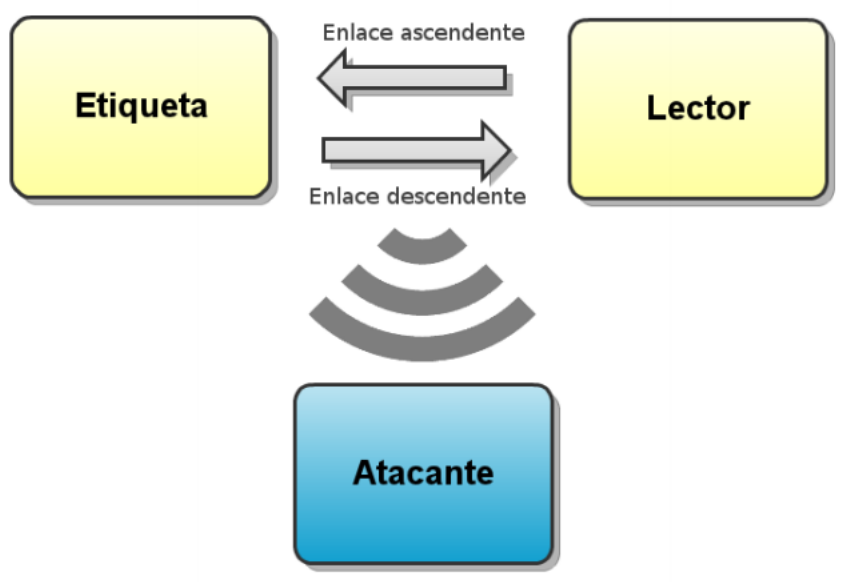
\includegraphics[width=0.5\textwidth]{figures/eavesdropping.png}
\end{figure}
%-----------
\subsection{Skimming}
Esta es la vulnerabilidad que atacaremos nosotros en el proyecto, consiste en obtener toda la información del sistema de la víctima y replicarlo en donde el atacante quiera. En esencia, la clonación.
\begin{figure}[!h]
	\centering
	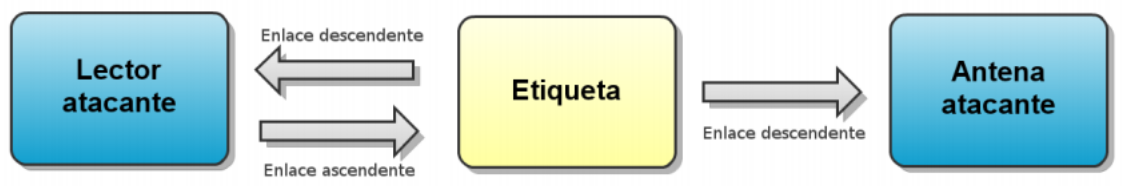
\includegraphics[width=0.5\textwidth]{figures/skimming.png}
\end{figure}
%-----------
\subsection{Denial of Service}
Como en muchas otras disciplinas, en el campo de las NFC también es posible hacerle a la víctima una denegación de servicio saturando el sistema y llenándolo de ruido.
\begin{figure}[!h]
	\centering
	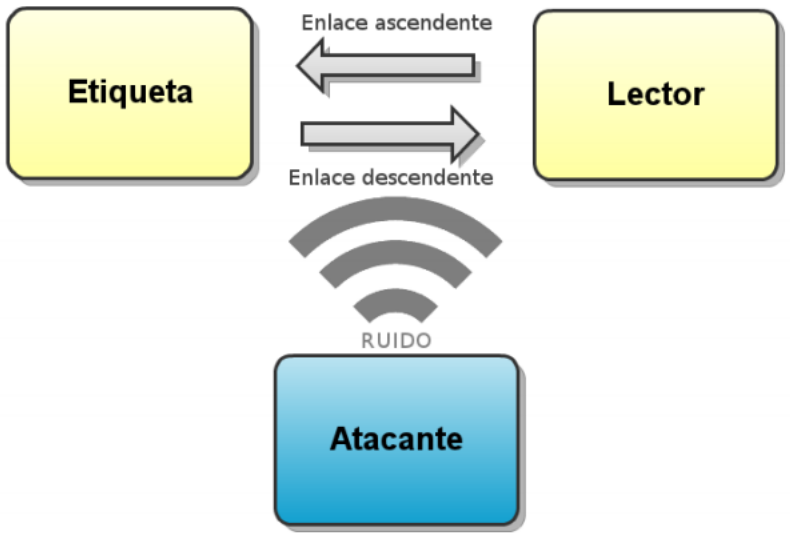
\includegraphics[width=0.4\textwidth]{figures/dos.png}
\end{figure}
%-----------
\subsection{Modificación de datos}
Este ataque consiste en modificar alguno -o todos- de los datos con los que actualmente cuenta la tarjeta. Esto puede utilizarse para el beneficio del sistema, por ejemplo recargar alguna tarjeta monedero, o para corromperla, insertando un chorro de unos.
\begin{figure}[!h]
	\centering
	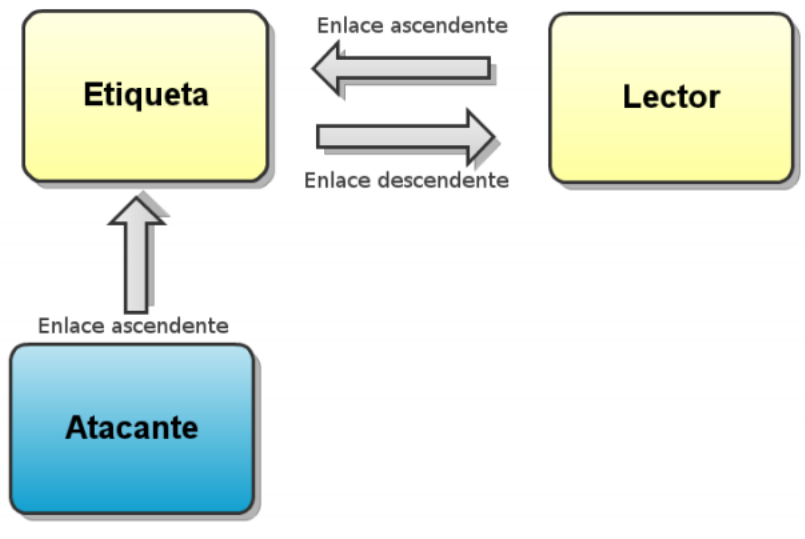
\includegraphics[width=0.4\textwidth]{figures/modificacion.png}
\end{figure}
%-----------
\subsection{Inserción de datos}
La inserción de datos se basa en sustituir el mensaje que la víctima manda por la que el atacante desee.
\begin{figure}[!h]
	\centering
	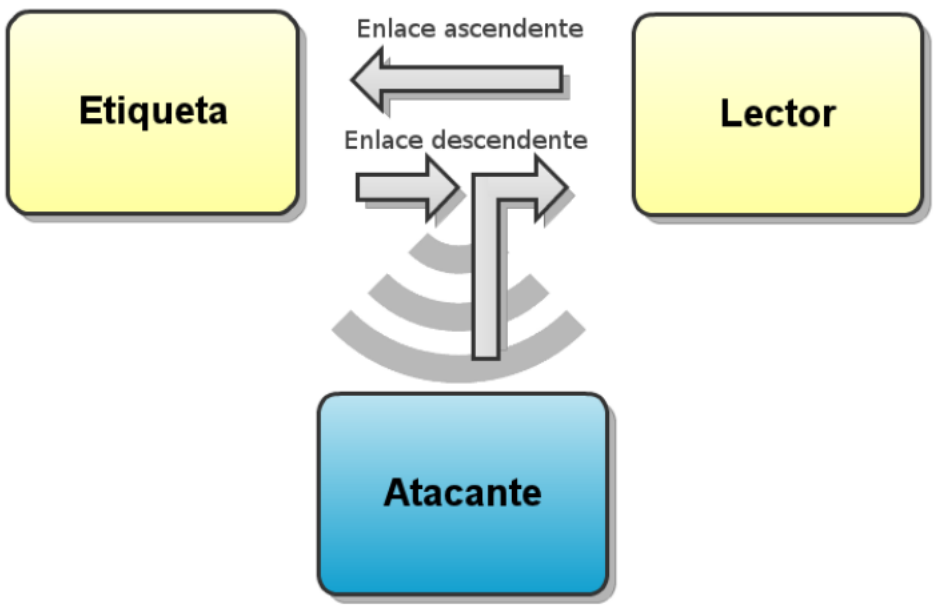
\includegraphics[width=0.5\textwidth]{figures/insercion.png}
\end{figure}
%-----------
\subsection{Man-in-the-middle}
En el proceso de man-in-the-middle se basa en interceptar los mensajes y después mandarlo modificados o igual que como la víctima los intercepta.
\begin{figure}[!h]
	\centering
	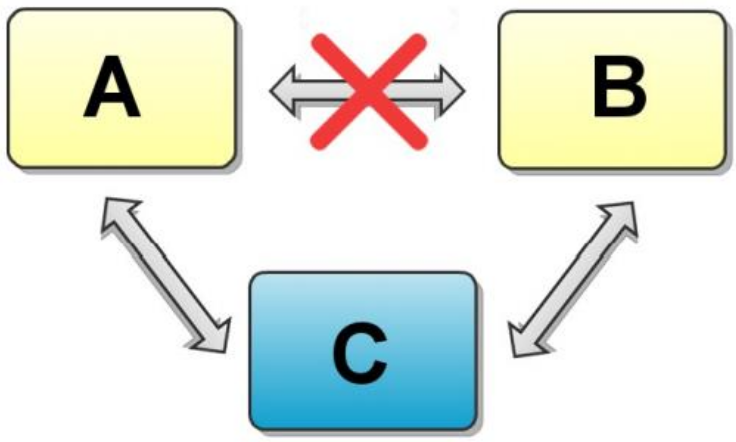
\includegraphics[width=0.5\textwidth]{figures/man.png}
\end{figure}


